\documentclass[11pt]{article}
\usepackage{amsmath} % Math
\usepackage{amssymb} % Math symbols
\usepackage[english]{babel} % Language
\usepackage{fancyhdr} % Header
\usepackage[a4paper, total={15cm, 20cm}]{geometry} % Dimensions of the paper and the text area
\usepackage[utf8]{inputenc} % encoding in UTF, needed for umlauts if German
\usepackage{mathtools} % Text above arrows
\usepackage{msc} % Drawing MSCs
\usepackage{multicol} % Multiple columns
\usepackage[explicit]{titlesec} % Automatic section titles
\usepackage{tikz} % Diagrams
\usetikzlibrary{arrows.meta, automata, shapes, matrix}
\usepackage{enumitem}   % Enumeration item


% Other packages that might be useful in the future
%\usepackage{lingmacros}
%\usepackage{tree-dvips}
%\usepackage{ulem}
%\usepackage{amsthm}
%\usepackage{amsbsy}
%\usepackage{textcomp,gensymb}
%\usepackage{graphicx}
%\usepackage{mathtools}

% Custom variant of msc environment:
% - No "msc" keyword, longer partial messages
% - Increased vertical distance between messages
% - Less distance to the frame left and right
% - Less distance between header and processes
% - Less distance between footer and frame
% - Passing all given options down to the msc environment
\newenvironment{cmsc}[1][]{\msc[msc keyword={}, self message width=1.1cm, level height=0.6cm, environment distance=1.2cm, head top distance=0.75cm, foot distance=0.5cm, #1]}{\endmsc}

% No indentation at new paragraphs
\setlength{\parindent}{0pt}

% Distance between columns
\setlength{\columnsep}{1cm}
% Vertical line between columns
\setlength{\columnseprule}{0.5pt}
\def\columnseprulecolor{\color{gray}}

% Settings
\newcommand{\sheetNr}{1}

%% Header
\fancyhf{}
\pagestyle{fancy}
\lhead{Model Checking Exercise Sheet \sheetNr}
\rhead{Aaron Grabowy: 345766\\ Timo Bergerbusch: 344408}
\setlength{\headheight}{28pt}

%% Automatic section titles
\titleformat{\section}{\normalfont\Large\bfseries}{}{0em}{Exercise #1}
\titleformat{\subsection}{\normalfont\large\bfseries}{}{0em}{#1)}

\begin{document}

\section{1}
\subsection{a}

The transition system TS$_1$ can be formally given as: $TS_1 = (S, Act, \rightarrow, AP, L)$ with:
\begin{itemize}
	\item $S = \{s_0,s_1,s_2,s_3, s_4\}$
	\item $Act = \{\alpha, \beta, \gamma \}$
	\item $\rightarrow = \{ (s_0, \gamma, s_1), (s_0, \alpha, s_2), (s_1, \gamma, s_1), (s_1, \alpha, s_3),(s_1, \beta, s_4), $\\
		  \hspace*{2cm} $s_2, \alpha, s_0), (s_2, \beta, s_4), (s_4, \alpha, s_2), (s_4, \gamma, s_3)  \} \subset S \times Act \times S$
	\item $S_0=\{s_0\}$
	\item $AP = \{a, b\}$
	\item $L: S \rightarrow 2^{AP}, s_0 \mapsto \{a\}, s_1 \mapsto \{a\}, s_2 \mapsto \{a,b\}, s_3 \mapsto \{b\}, s_4 \mapsto \{a,b\}$
\end{itemize}

\subsection{b}

\subsubsection{finite execution:} 
$$s_0 \xrightarrow{\alpha} s_2$$
\subsubsection{infinite execution:} 
$$s_0 \xrightarrow{\gamma} s_1 \xrightarrow{\gamma} s_1 \xrightarrow{\gamma} \dots$$


\subsection{c}

\begin{enumerate}[label=\roman*)]
	\item AP-deterministic: \\
		The given transition system $TS_1$ is AP-deterministic, since $|S_0|\le 1$ and there are no two transitions $t_1=(s, \eta , s'),= (s, \tau, s'') \in \rightarrow$, $\eta, \tau \in Act$, $s, s', s'' \in S$ ,such that $L(s') = L(s'')$
	\item action-deterministic: \\
		The given transition system $TS_1$ is action-deterministic, since $|S_0|\le 1$ and there are no two $t_1=(s, \eta , s'),= (s, \eta, s'') \in \rightarrow$, $\eta \in Act$, $s, s', s'' \in S$ with $s' \neq s''$
\end{enumerate}

\newpage
\section{2}

\subsection{a}

\begin{itemize}
	\item $\lambda_y = r_1 \land r_2$
	\item $\delta_{r_1} = (x \land \lnot r_1) \lor (r_1 \land \lnot x) = x \oplus r_1$
	\item $\delta_{r_2} = (\lnot x \land r_2) \lor (x \land r_1)$
\end{itemize}

\subsection{b}

% all, since x can vary and r1 and r2 can be arbitrarily initialized
%unclear
The state space can be given as all possible combinations of the values of $x, r_1$ and $r_2$.\\

$S = \{(x=0, r_1=0, r_2=0),(x=0, r_1=0, r_2=1),(x=0, r_1=1, r_2=0),$\\
	\hspace*{1cm}$(x=0, r_1=1, r_2=1),x=1, r_1=0, r_2=0),(x=1, r_1=0, r_2=1),$\\
    \hspace*{1cm}$(x=1, r_1=1, r_2=0),(x=1, r_1=1, r_2=1)\}$\\
	   
This is valid, since the we have to consider all possible inputs for $x$ which are 0 and 1, and
all the possible initial values of the registers $r_1$ and $r_2$.
										
\subsection{c}

	\begin{tikzpicture}[node distance = 3cm, every node/.style={rounded corners=.25cm}]
		\node[draw, label = above left:{\small $\emptyset$}] (n000) {$x=0, r_1=0, r_2=0$};
		\node[above = 0.5cm of n000] (dummy0) {};
		\node[draw, below = of n000, label = above left:{\small $\{r_1,y\}$}] (n010) {$x=0, r_1=1, r_2=0$};
		\node[draw, below = of n010, label = above left:{\small $\{r_2,y\}$}] (n001) {$x=0, r_1=0, r_2=1$};
		
		\node[draw, right = of n000, label = above right:{\small $\{x\}$}] (n100) {$x=1, r_1=0, r_2=0$};
		\node[above = 0.5cm of n100]          (dummy1) {};
		\node[draw, below = of n100, label = below right:{\small $\{x,r_1, y\}$}] (n110) {$x=1, r_1=1, r_2=0$};
		\node[draw, below = of n110, label = below right:{\small $\{x,r_2, y\}$}] (n101) {$x=1, r_1=0, r_2=1$};
		
		\node[draw, below = of n001, label = below right:{\small $\{r_2, y\}$}] (n011) {$x=0, r_1=1, r_2=1$};
		\node[draw, below = of n101, label = below right:{\small $\{x,r_2, y\}$}] (n111) {$x=1, r_1=1, r_2=1$};
		
		
		\draw[->, thick] (dummy0) edge (n000);	
		\draw[->, thick] (dummy1) edge (n100);	
		
		\path[->, thick] (n000) edge[loop left] (n000);	% first starting state
		
		% second starting state
		\path[->, thick] (n100) edge                  (n010); % to 1
		\path[->, thick] (n100) edge                  (n110); % to 2
		
		% from 1
		\path[->, thick] (n010) edge[loop below]      (n010); % to 1
		\path[->, thick] (n010) edge                  (n110); % to 2
		
		% from 2
		\path[->, thick] (n110) edge                  (n001); % to 3
		\path[->, thick] (n110) edge[bend left = 20]  (n101); % to 4
		
		%from 3
		\path[->, thick] (n001) edge[loop below]      (n001); % to self
		\path[->, thick] (n001) edge                  (n101); % to 4
		
		%from 4
		\path[->, thick] (n101) edge                  (n010); % to 1
		\path[->, thick] (n101) edge[bend left = 20]  (n110); % to 2
		
		% non-reachable
		
		%from 5
		\path[->, thick] (n011) edge[loop below]      (n011); % to self
		\path[->, thick] (n011) edge[bend left = 00]  (n111); % to 6
		
		%from 6
		\path[->, thick] (n111) edge                  (n001); % to 3
		\path[->, thick] (n111) edge                  (n101); % to 4
	\end{tikzpicture}

\subsection{d}
The set $Reach(TS)$ follows from c) with:\\
$ Reach(TS)= \{(x=0, r_1=0, r_2=0), (x=1, r_1=0, r_2=0), \\ 
		\hspace*{2.6cm}(x=0, r_1=1, r_2=0), (x=1, r_1=1, r_2=0), \\
		\hspace*{2.6cm}(x=0, r_1=0, r_2=1), (x=1, r_1=0, r_2=1)\}$
\section{3}

\subsection{a}

\begin{tikzpicture}[node distance = 3cm, every path/.style={->, thick}]
	\node[ellipse, draw]                (l0) {$l_0$} ;
	\node[above =0.5cm of l0]           (dummy) {};
	\node[ellipse, draw, right = of l0] (l1) {$l_1$} ;
	\node[ellipse, draw, right = of l1] (l2) {$l_2$} ;
	\node[ellipse, draw, below = of l1] (l3) {$l_3$} ;
	\node[ellipse, draw, left = of l3]  (l4) {$l_4$} ;
	
	\draw[->, thick] (dummy) edge (l0);	
	\draw[->, thick] (l0) edge                   node[above]               {$b[i]\coloneqq false$}                   (l1);	
	\path (l1) edge [bend left = 20]             node[above]               {$k != i:$}                               (l2);
	\path (l1) edge                              node[right]               {$k=i$}                                   (l3);	
	\path (l2) edge [loop right]                 node[right, align = center] {$\text{not }b[1-i]:$\\ $k\coloneqq i$} (l2);
	\path (l2) edge [bend left = 20]             node[below]               {$b[1-i]:$}                               (l1);	
	\path (l3) edge                                                                                                  (l4);	
	\path (l4) edge                              node[left]                {$b[i] \coloneqq true$}                   (l0);
\end{tikzpicture}

\subsection{b}

\begin{tikzpicture}[node distance = 2cm, every node/.style={rounded corners=.25cm}, every path/.style={->, thick}]

\end{tikzpicture}

\end{document}
